\appendix

\chapter{General relativity}

\section{The geometry of curved spacetime}
\label{chap:gr_summary} % TODO: chap -> sec

\newcommand\pdvx[2]{\pdv{x^{#1}}{x^{#2}}}

In this appendix, we review the geometrical aspects of general relativity.
We make no attempt to be mathematically rigorous, but rather focus on listing important quantities and equations and the intuitive connection between them.
For more details, we refer to detailed books and notes on the subject such as \cite{ref:carroll}, \cite{ref:mika_gr_notes} and \cite{ref:mtw}, all of whom this summary is based on.

\subsection{Coordinates and tensors}

In general relativity, $3$-dimensional space and $1$-dimensional time are no longer regarded separate as they are in Newtonian mechanics.
They are rather intertwined into \emph{spacetime} -- a $(3+1)$-dimensional construct with \textbf{coordinates}
% position is just "coordinates", not a 4-vector: https://physics.stackexchange.com/questions/192886/does-spacetime-position-not-form-a-four-vector
\begin{equation}
	x^\mu = (x^0, x^1, x^2, x^3) .
\end{equation}
In flat Minkowski space, the coordinates could be taken as $x^\mu = (ct, x, y, z)$.
Mathematically, the geometry of spacetime is described by a \emph{Riemannian manifold} that generalizes flat Minkowski space to \emph{curved space}.
At every point on such a manifold, spacetime locally resembles Minkowski space in the \emph{tangent space} located at that point, and all such tangent spaces vary in a smooth manner from point to point.
For example, \cref{fig:tangent_space} pictures the tangent space at a point of the $2$-sphere manifold.
Familiar concepts like angles, lengths, area and volume apply locally in the tangent space at each point in infinitesimal form, and one can generalize such concepts to the full manifold by integrating the local contributions from one point on the manifold to another.

\begin{figure}
\centering
\includesvg[width=0.60\textwidth]{figures/tangent-space.svg}
\caption{\label{fig:tangent_space}The tangent space at a point on the $2$-sphere manifold can be pictured as the tangent plane at that point. If a vector field is placed on the manifold, the vector would lie in this tangent space. Illustration by \cite{ref:figure_tangent_space}.}
\end{figure}

% transformation law inspiration: https://math.stackexchange.com/a/958524 and Wikipedia: "holonomic basis"

\newcommand\lincombo[1]{\left( a \odv{#1}{\tau} + b \odv{#1}{\lambda} \right)}
\newcommand\lincomboslash[1]{\left( a \odv{#1}/{\tau} + b \odv{#1}/{\lambda} \right)}
We will place vector fields $V^\mu(x^\nu)$, and later tensor fields, that associate a vector $V^\mu$ to every point $x^\nu$ on a manifold.
As explained in \cref{fig:tangent_space}, such a vector lies in the tangent vector space at every point on the manifold.
To motivate the transformation properties of tensors on a manifold, we can use the fact that the set of directional derivatives constitute a vector space with basis vectors given by the partial derivatives. 
Suppose $\phi(x)$ is a scalar function and $x(\tau)$ and $x(\lambda)$ are two paths on the manifold with directional derivatives given through the chain rule as
\begin{equation}
	\odv{\phi}{\tau} = \odv{x^\mu}{\tau} \partial_\mu \phi
	\qquad \text{and} \qquad
	\odv{\phi}{\lambda} = \odv{x^\mu}{\lambda} \partial_\mu \phi .
\end{equation}
Then the linear combination $\lincomboslash{}$ is also a perfectly good derivative operator, as it is both linear and satisfies the product rule
\begin{equation}
	\lincombo{}(fg) = \ldots = \lincombo{f} g + \lincombo{g} f .
\end{equation}
One can verify that the set of all differential operators, implicitly assumed to work on some scalar function, satisfy all criteria for being a vector space.
Thus, like one can regard $\vec{V} = V^\mu \vec{e}_\mu$ as a vector with components $V^\mu$ and basis vectors $\vec{e}_\mu$, one can regard
\begin{equation}
	\odv{}{\lambda} = \odv{x^{\mu}}{\lambda} \partial_{\mu} 
\end{equation}
as a vector with components $\odv{x^{\mu}}/{\lambda}$ and basis vectors $\partial_\mu$.
To see this clearly, make a coordinate transformation
\begin{equation}
	x \rightarrow x'(x)
	\qquad \text{with inverse} \qquad
	x' \rightarrow x(x')
	\qquad \text{and Jacobians} \qquad
	\pdv{x'^{\alpha}}{x^\gamma} \pdv{x^{\gamma}}{x'^{\beta}} = \delta^{\alpha}_{\beta} .
	\label{eq:gr_summary:coordinate_transformation}
\end{equation}
Using the chain rule and the Jacobian property, the directional derivative transforms as
\begin{equation}
	\odv{}{\lambda} = \odv{x^{\mu'}}{\lambda} \partial_{\mu'} = \underbrace{\Bigg( \odv{x^{\alpha}}{\lambda} \pdvx{\mu'}{\alpha} \Bigg)}_\text{components} \underbrace{\Bigg( \pdvx{\beta}{\mu'} \partial_{\beta} \Bigg)}_\text{basis} = \odv{x^{\mu}}{\lambda} \partial_{\mu} .
\end{equation}
We see that the transformation of the components and the basis vectors exactly cancel each other, so the directional derivative is unchanged -- consistent with it being a vector.

Note that we adopted the convention $x^{\mu'} = x'^\mu$ of placing the prime on the \emph{index} rather than the underlying object, but defined to mean the same.
The benefit is that an index transforms with the partial derivative that has the primed coordinate in the \emph{same position as the index}, so we can always deduce the right transformation by simply staring at the expression.
%If there is a prime on an index, it means that a coordinate transformation has been applied to that index.
%The benefit of this is that an index transforms with the partial derivative that has the primed coordinate in the \emph{same position as the index} -- upper indices go with primed coordinates in the numerator, and lower indices with primes in the denominator.
%In addition, we are free to ``reuse'' the same index twice -- once as a free index, and once for the contraction.
%With this convention, we can always deduce the correct transformation laws from the index position, and we can place remaining indices so that they are contracted to yield an expression with the right number of free indices.

We define an $n$-dimensional \textbf{covariant vector} as an $n$-tuple $V_\mu$ that transforms with the \emph{same} matrix $\pdv{x^{\mu}}/{x^{\mu'}}$ as the change of basis as
\begin{equation}
	V_{\mu'} = \pdv{x^{\mu}}{x^{\mu'}} V_\mu .
	\label{eq:covariant_transformation}
\end{equation}
Oppositely, we define an $n$-dimensional \textbf{contravariant vector} as an $n$-tuple $V^\mu$ that transforms with the \emph{inverse} matrix $\pdv{x^{\mu'}}/{x^{\mu}}$ as
\begin{equation}
	V^{\mu'} = \pdv{x^{\mu'}}{x^\mu} V_\mu .
	\label{eq:contravariant_transformation}
\end{equation}
More generally, we define a $n$-dimensional \textbf{tensor} of rank $(r,s)$ as an array composed of $r$ $n$-dimensional contravariant indices and $s$ $n$-dimensional covariant indices that transforms as
\begin{equation}
	T^{\mu_1' \dots \mu_r'}_{\nu_1' \dots \nu_s'} = \pdv{x^{\mu_1'}}{x^{\mu_1}} \cdots \pdv{x^{\mu_r'}}{x^{\mu_r}}
	                                                \pdv{x^{\nu_1}}{x^{\nu_1'}} \cdots \pdv{x^{\nu_s}}{x^{\nu_s'}}
												    T^{\mu_1 \dots \mu_r}_{\nu_1 \dots \nu_s}
	\label{eq:tensor_transformation}
\end{equation}
under the coordinate transformation \eqref{eq:gr_summary:coordinate_transformation}.

\iffalse
We will work with vector fields $V^\mu(x)$ on manifolds.
To each point on $x$ on the manifold, we associate a tangent vector $V^\mu(x)$.
How do vectors, and generally tensors, transform under a change of coordinates $x' = x'(x)$ on the manifold?
First, note that \emph{directional derivatives} constitute a vector space when acting on scalar functions.
Imagine two curves $x^\mu(\tau)$ and $x^\nu(\lambda)$ with directional derivatives $\odv{}/{\tau}$ and $\odv{}/{\lambda}$.
The linear combination $a \odv{}/{\tau} + b \odv{}/{\lambda}$ is also in the same space, as
\begin{equation}
	\lincombo{}(fg) = \ldots = \lincombo{f} g + \lincombo{g} f
\end{equation}
so the Leibniz rule is satisfied and the linear combination is also a proper derivative operator.
By the chain rule,
\begin{equation}
	\odv{}{\lambda} = \odv{x^\mu}{\lambda} \partial_\mu ,
\end{equation}
so the partial derivatives $\partial_\mu$ in fact constitute a natural basis for this vector space.
Since these are the basis vectors, we can deduce the transformation laws by requiring that $V^\mu \partial_\mu$ be constant under a change of coordinates:
\begin{equation}
	V^\mu \partial_\mu = V^{\mu'} \partial_{\mu'} = V^{\mu'} \pdv{x^\mu}{x^{\mu'}} \partial_\mu ,
\end{equation}
so the general \textbf{transformation law for contravariant vectors} is
\begin{equation}
	V^{\mu'} = \pdv{x^{\mu'}}{x^\mu} V_\mu .
\end{equation}

To get the transformation law for covariant vectors, we make use of the gradient of a scalar function
\begin{equation}
	\nabla \phi = \partial_\mu \phi \vec{e}^\mu 
\end{equation}
Using the chain rule,
\begin{equation}	
	\partial_{\mu'} \phi = \pdv{x^\mu}{x^{\mu'}} \partial_\mu \phi ,
\end{equation}
so the \textbf{transformation law for covariant vectors} is
\begin{equation}
	V_{\mu'} = \pdv{x^{\mu}}{x^{\mu'}} V_\mu .
\end{equation}
This line of reasoning can be extended to find the \textbf{general transformation law for tensors} (where we suppress the ordering of the indices)
\begin{equation}
	T^{\mu_1' \dots \mu_m'}_{\nu_1' \dots \nu_n'} = \pdv{x^{\mu_1'}}{x^{\mu_1}} \cdots \pdv{x^{\mu_m'}}{x^{\mu_m}}
	                                                \pdv{x^{\nu_1'}}{x^{\nu_1}} \cdots \pdv{x^{\nu_n'}}{x^{\nu_n}}
												    T^{\mu_1 \dots \mu_m}_{\nu_1 \dots \nu_n}
\end{equation}
\fi

\subsection{Metric tensor}

The \textbf{metric tensor}
\begin{equation}
	g\indices{_\mu_\nu}(x) = \vec{e}_\mu(x) \cdot \vec{e}_\nu(x)
\end{equation}
is defined as the inner products between basis vectors $\vec{e}_\mu$ that span the tangent spaces at each point $x$ on the manifold.
It thus encodes the lengths vectors of the basis vectors and angles between them and is a fundamental object that describes the geometry of the manifold.

We define the \textbf{inverse metric tensor} $g^{\mu \nu}$ as the inverse matrix satisfying
\begin{equation}
	g^{\mu \nu} g_{\nu \sigma} = \delta^\mu_\sigma .
\end{equation}
Using the metric and its inverse, we can \textbf{raise and lower indices} on tensors.
For example, the object $g_{\mu \nu} V^\nu$, according to definition \eqref{eq:tensor_transformation}, transforms as a covariant vector
\begin{equation}
	g_{\mu' \nu'} V^{\nu'} = \left( \pdvx{\alpha}{\mu'} \pdvx{\beta}{\nu'} g_{\alpha \beta} \right) \left( \pdvx{\nu'}{\nu} V^{\nu} \right) = \pdvx{\alpha}{\mu'} g_{\alpha \nu} V^\nu ,
\end{equation}
so it is meaningful to label it as a covariant vector with a lower index $V_\mu = g_{\mu \nu} V^\nu$.
Similarly, we can use the inverse metric $g^{\mu \nu}$ to raise indices.
As this argument only relied on the defining transformation law \eqref{eq:tensor_transformation}, it is clear that any tensor of rank $(2,0)$ or $(0,2)$ would suffice to raise or lower indices.
But the metric is the most natural choice, as it is inherent to the manifold and always available to us.

\subsection{Line element and volume}

From the metric tensor, one defines the \textbf{line element}
\begin{equation}
	\dif s = \sqrt{g\indices{_\mu_\nu} \dif x^\mu \dif x^\nu}
	\label{eq:def_line_elem}
\end{equation} 
that extends the concept of distance locally to every point on the manifold.
By integrating the line element from one point on the manifold to another, one can compute the total distance
\begin{equation}
	s = \int_1^2 \dif s = \int_1^2 \sqrt{g\indices{_\mu_\nu} \dif x^\mu \dif x^\nu}
\end{equation}
between the points.
Similarly, one can compute the \textbf{volume} of a region
\begin{equation}
	V = \int \dif V = \int \sqrt{\det{\gamma}} \dif x^1 \dif x^2 \dif x^3 ,
\end{equation}
where $\gamma$ is the induced metric on the surface and $\det{\gamma}$ its determinant.
The factor $\sqrt{\det{\gamma}}$ arises to make the volume element $\dif^n x \sqrt{\det{\gamma}}$ invariant under coordinate transformations.

\subsection{Covariant derivatives and connection coefficients}

Knowing how vectors and general tensors transform, let us generalize the notion of a derivative to curved space.
By the transformation rules we have found so far, the normal partial derivative of a vector transforms as
\begin{equation}
	\partial_{\mu'} V^{\nu'} = \bigg( \pdvx{\mu}{\mu'} \partial_\mu \bigg) \bigg( \pdvx{\nu'}{\nu} V^\nu \bigg)
	                         = \pdvx{\mu}{\mu'} \pdvx{\nu'}{\nu} \partial_\mu V^\nu + \pdvx{\mu}{\mu'} \pdv{x^{\nu'}}{x^\mu, x^\nu} V^\nu .
\end{equation}
The first term respects the tensor transformation law \eqref{eq:tensor_transformation}, but the second does not, so $\partial_\mu V^\nu$ is \emph{not} a tensor.
We define a tensorial derivative $\nabla_\mu$ that by demanding that it transforms as
\begin{equation}
	\nabla_{\mu'} V^{\nu'} = \pdvx{\mu}{\mu'} \pdvx{\nu'}{\nu} \nabla_\mu V^\nu .
\label{eq:gr_summary:covariant_derivative_demand}
\end{equation}
It turns out that our requirements can be met if we define the \textbf{covariant derivative} as
\begin{equation}
	\nabla_\mu V^\nu = \partial_\mu V^\nu + \Gamma_{\sigma \mu}^\nu V^\sigma .
	%\qquad \text{or} \qquad
	%\nabla_\mu V_\nu = \partial_\mu V_\nu - \Gamma_{\nu \mu}^\sigma V_\sigma ,
\end{equation}
It is possible to show that it obeys the tensorial transformation \eqref{eq:gr_summary:covariant_derivative_demand} if the so-called \textbf{connection coefficients} $\Gamma_{\sigma _\mu}^\nu$ transform according to \cite[equation 3.6-3.10]{ref:carroll} 
\begin{equation}
	\Gamma^{\nu'}_{\mu' \lambda'} = \pdvx{\mu}{\mu'} \pdvx{\lambda}{\lambda'} \pdvx{\nu'}{\nu}  \Gamma^{\nu}_{\mu \lambda} + \pdvx{\mu}{\mu'} \pdvx{\lambda}{\lambda'} \pdv{x^{\nu'}}{x^\mu, x^\lambda} .
	\label{eq:connection_transformation}
\end{equation}
It is possible to generalize the covariant derivative to an arbitrary tensor $T^{\alpha_1 \ldots \alpha_r}_{\beta_1 \ldots \beta_s}$ of rank $(r,s)$ (where we suppress the order of the indices) by adding more terms with connection coefficients.
The general \textbf{covariant derivative} that respects the tensorial transformation law \eqref{eq:tensor_transformation} turns out to be \cite[equation 3.11-3.16]{ref:carroll}
\begin{equation}
\begin{split}
	\nabla_\mu T^{\alpha_1 \ldots \alpha_r}_{\beta_1 \ldots \beta_s} &= \partial_\mu T^{\alpha_1 \ldots \alpha_r}_{\beta_1 \ldots \beta_s} \\
	                                                                 &+ \Gamma^{\alpha_1}_{\sigma\mu} T^{\sigma \alpha_2 \ldots \alpha_r}_{\beta_1 \ldots \beta_s} + \dots + \Gamma^{\alpha_r}_{\sigma\mu} T^{\alpha_1 \ldots \alpha_{r-1}\sigma}_{\beta_1 \ldots \beta_s} \\
	                                                                 &- \Gamma^\sigma_{\beta_1 \mu} T^{\alpha_1 \ldots \alpha_r}_{\sigma \beta_2 \ldots \beta_s} - \cdots - \Gamma^\sigma_{\beta_s \mu} T^{\alpha_1 \ldots \alpha_r}_{\beta_1 \ldots \beta_{s-1} \sigma} .
	\label{eq:def_cov_deriv}
\end{split}
\end{equation}
That is, for each upper index $\alpha_i$, add $+\Gamma^{\alpha_i}_{\sigma \mu} T^{\alpha_1 \ldots \alpha_{i-1} \sigma \alpha_{i+1} \ldots \alpha_r}_{\beta_1 \ldots \beta_s}$,
and for each lower index $\beta_i$, add $-\Gamma^{\sigma}_{\beta_i \mu} T^{\alpha_1 \ldots \alpha_r}_{\beta_1 \ldots \beta_{i-1} \sigma \beta_{i+1} \ldots \beta_s}$,

Note that the connection coefficients \eqref{eq:connection_transformation} \emph{do not} transform like tensors -- the whole point is to stash the non-tensorial behavior into the connection coefficients so that the \emph{covariant derivative} transforms as a tensor.
However, since $\nabla_\mu V^\nu$ and $\hat{\nabla}_\mu V^\nu$ for two different connection coefficients $\Gamma^\alpha_{\beta \mu}$ and $\hat{\Gamma}^\alpha_{\beta \mu}$ by definition are tensors, the \emph{difference}
\begin{equation}
	S\indices{^\alpha_\beta_\gamma} = \Gamma^\alpha_{\beta \gamma} - \hat{\Gamma}^\alpha_{\beta \gamma}
\end{equation}
between two connection coefficients \emph{does} transform like a tensor.

There are many possible choices of the connection coefficients that satisfy \cref{eq:connection_transformation}.
However, it turns out that we can find a set of \emph{unique} connection coefficients from the \emph{metric} if we impose two additional requirements.
First, we demand that the \textbf{torsion tensor}
\begin{equation}
	T\indices{^\alpha_\beta_\gamma} = \Gamma^\alpha_{\beta\gamma} - \Gamma^\alpha_{\gamma\beta}
	\label{eq:torsion_tensor}
\end{equation}
vanishes.
Equivalently, the connection coefficients $ \Gamma^\alpha_{\beta\gamma} = \Gamma^\alpha_{\beta\gamma} $ are symmetric in the lower indices.
Second, we require \textbf{metric compatibility}
\begin{equation}
	\nabla_\rho g_{\mu \nu} = 0 .
\end{equation}
This implies that
\begin{equation}
	g_{\mu \lambda} \nabla_\rho V^\lambda = \nabla_\rho (g_{\mu \lambda} V^\lambda) = \nabla_\rho V_\mu ,
\end{equation}
so we do not have to be overly careful regarding index placement when taking covariant derivatives.
Using both of these assumptions, we can write out three metric compatibility requirements
\newcommand\metriccompatibilityequation[3]{\nabla_{#1} g_{{#2}{#3}} &= \partial_{#1} g_{{#2}{#3}} - \Gamma^\lambda_{{#1}{#2}} g_{\lambda {#3}} - \Gamma^\lambda_{{#1}{#3}} g_{{#2} \lambda} = 0}
\begin{align}
	\metriccompatibilityequation{\rho}{\mu}{\nu} \\
	\metriccompatibilityequation{\mu}{\nu}{\rho} \\
	\metriccompatibilityequation{\nu}{\rho}{\mu} .
\end{align}
By subtracting the second and third equation from the first and solving the resulting equation for the connection, we find the \textbf{Christoffel symbols} or \textbf{metric connection}
\begin{equation}
	\Gamma^\sigma_{\mu \nu} = \frac{1}{2} g\indices{^\sigma^\rho} \left(
		\partial\indices{_\mu} g\indices{_\nu_\rho} +
		\partial\indices{_\nu} g\indices{_\rho_\mu} -
		\partial\indices{_\rho} g\indices{_\mu_\nu}
	\right) .
	\label{eq:def_christoffel}
\end{equation}
In general relativity, we will \emph{always} use this unique representation of the connection coefficients given in terms of the metric only.
With this choice, the metric single-handedly determines the geometry of spacetime, as it is the only fundamental object that all the other geometric quantities we have looked at depends on.

\TODO{gjør et ``dypdykk'' for å finne ut om det er mulig å gjøre GR \emph{uten} $0$ torsion og metric compatibility}

\iffalse
\begin{align}
	\nabla_c T\indices{^{a_1 \ldots a_r}_{b_1 \ldots b_s}} &= \partial_c {T^{a_1 \ldots a_r}}_{b_1 \ldots b_s} \\
	                                                       &+ \Gamma^{a_1}_{dc} T\indices{^{d a_2 \ldots a_r}_{b_1 \ldots b_s}} + \dots + \Gamma^{a_r}_{dc} T\indices{^{a_1 \ldots a_{r-1}d}_{b_1 \ldots b_s}} \\
	                                                       &- {\Gamma^d}_{b_1 c} {T^{a_1 \ldots a_r}}_{d b_2 \ldots b_s} - \cdots - {\Gamma^d}_{b_s c} {T^{a_1 \ldots a_r}}_{b_1 \ldots b_{s-1} d}.
	\label{eq:def_cov_deriv}
\end{align}
\fi

\subsection{Parallel transport and geodesic equation}
\label{sec:geodesic}

\begin{figure}
\centering
\includesvg[width=0.5\textwidth]{figures/parallel_transport.svg}
\caption{\label{fig:parallel_transport}When a vector is parallel transpored around a closed loop on the $2$-sphere, its final direction depends on the path taken. Illustration by \cite{ref:figure_parallel_transport}.}
\end{figure}

Now that we know how to take proper derivatives of vector fields and general tensor fields on manifolds, we can discuss how to parallel transport vectors on the manifold.
In flat space, we can move a vector around and keep its Cartesian components constant to parallel transport it.
But on a curved $2$-sphere, a vector that is parallel transported will end up being different depending on the route taken, as illustrated in \cref{fig:parallel_transport}.
Generalizing the directional derivative $\odv{}/{\tau} = (\odv{x^\mu}/{\tau}) \partial_\mu$ from calculus, we define the \textbf{directional covariant derivative} along a path $x(\tau)$ as
\begin{equation}
	\frac{D}{\mathrm{d} \tau} = \odv{x^\mu}{\tau} \nabla_\mu,
\end{equation}
where $\nabla_\mu$ is the covariant derivative \eqref{eq:def_cov_deriv}.
We say that a tensor is parallel transported if its components are kept constant during transport, as expressed by
\begin{equation}
	\frac{D}{\mathrm{d} \tau} T^{\mu_1 \ldots \mu_m}_{\nu_1 \ldots \nu_n} = 0 .
\end{equation}
For the special case of a vector $V^\mu$ we get the \textbf{equation of parallel transport}
\begin{equation}
	\odv{V^\mu}{\tau} + \Gamma^{\mu}_{\sigma \rho} \odv{x^\sigma}{\tau} V^\rho = 0 .
	\label{eq:parallel_transport}
\end{equation}
The solution of this first order differential equation is the continuation $V^\mu(\tau)$ from an initial vector $V^\mu(0)$ along the path such that its components are constant.

In Euclidean space, a straight line is the shortest path between two points.
In curved space, we call the shortest path between two points on a manifold a \textbf{geodesic}.
An equivalent definition of both a straight line and a geodesic is that it is the path $x(\tau)$ that parallel transports its own tangent vector $\odv{x^\mu}/{\tau}$.
Inserted into the equation of parallel transport \eqref{eq:parallel_transport}, we find the \textbf{geodesic equation}
\begin{equation}
	\odv[2]{x^\mu}{\tau} + \Gamma^\mu_{\rho \sigma} \odv{x^\rho}{\tau} \odv{x^\sigma}{\tau} = 0 .
	\label{eq:geodesic}
\end{equation}
In flat space, it reduces to the equation of a straight line $\odv[2]{x^\mu}/{\tau} = 0$.
One of Einstein's profound insights of general relativity was that gravity does not simply alter the path of a freely falling particle away from the straight line it would follow in Euclidean space in the abscence of gravity.
Instead, gravity presents itself in the geometry of spacetime, as the presence of energy-momentum curves spacetime and lays geodesic ``tracks'' according to \cref{eq:geodesic} that any freely falling particle is destined to follow.
\emph{Gravity is geometry}.

\subsection{Riemann curvature tensor, Ricci tensor and Ricci scalar}

% motivate by connecting it to the metric? 
% https://math.stackexchange.com/a/1213124 
% https://math.stackexchange.com/q/884794 
% https://math.stackexchange.com/q/2896648
% https://en.wikipedia.org/wiki/Ricci_curvature#Direct_geometric_meaning (taylor expansion around normal coords) 

So far we have used the term ``curvature'' quite informally -- let us now formalize this.
We already saw that parallel transporting a vector along different paths on a curved manifold like the $2$-sphere yield different results.
We have also seen that the covariant derivative measures the rate of change of a vector along some direction compared to what it would've been if it was parallel transported.
Thus, the commutator $[ \nabla_\mu, \nabla_\nu ] V^\rho = \nabla_\mu V^\rho - \nabla_\nu V^\rho$ measures the difference of parallel transporting a vector along the two different directions.
Using \cref{eq:def_cov_deriv}, it turns out we can write this as
\begin{equation}
	[ \nabla_\mu, \nabla_\nu ] V^\rho = R\indices{^\rho_{\sigma \mu \nu}} V^\sigma - T\indices{^\lambda_{\mu \nu}} \nabla_\lambda V^\rho ,
\end{equation}
where $T\indices{^\lambda_{\mu \nu}}$ is the torsion tensor \eqref{eq:torsion_tensor} that we assume to vanish and we define the \textbf{Riemann curvature tensor}
\begin{equation}
	R\indices{^\rho_\sigma_\mu_\nu} =
	\partial\indices{_\mu} \Gamma^\rho_{\nu \sigma} -
	\partial\indices{_\nu} \Gamma^{\rho}_{\mu \sigma} +
	\Gamma^\rho_{\mu \lambda} \Gamma^{\lambda}_{\nu \sigma} -
	\Gamma^\rho_{\nu \lambda} \Gamma^{\lambda}_{\mu \sigma} .
	\label{eq:def_riemann_tensor}
\end{equation}
We expect that if space is flat, then a parallel transported vector should not depend on the path, so the commutator and thus the Riemann tensor should vanish.
If there exists \emph{any} choice of coordinates in which the curvature tensor vanishes, then it vanishes in \emph{all} coordinates by its tensorial nature, and this is our ultimate definition of \textbf{flat space}.
In fact, it turns out that at any point $x_0$ we can find \textbf{normal coordinates} $x^\mu$ in which the metric locally resembles that of flat space with $g_{\mu \nu} = \eta_{\mu \nu}$ and $\partial_\sigma g_{\mu \nu} = 0$ to first order in the displacement.
To second order in the displacement, \cite{ref:metric_taylor_expansion} shows that the metric can be written
\begin{equation}
	g_{\mu \nu}(x) = \eta_{\mu \nu} - \frac12 R_{\alpha \mu \beta \nu} (x^\alpha - x_0^\alpha) (x^\beta - x_0^\beta) .
\end{equation}
This shows that the Riemann tensor is a \emph{very} appropriate measure of curvature.

% TODO: motivate
% https://en.wikipedia.org/wiki/Introduction_to_the_mathematics_of_general_relativity#Curvature_tensor (need two indices to enter the Einstein field equations -- "geometry" = metric comes with 2 indices, and "energy-momentum" come with 2 indices, https://physics.stackexchange.com/a/220650)
% see great motivation at https://physics.stackexchange.com/a/220650
% and great motivation at https://physics.stackexchange.com/a/219682

From the curvature tensor, we can form tensors of lower rank by contracting some of its indices.
We know that the energy-momentum tensor $T^{\mu \nu}$ that enter the Einstein field equations \eqref{eq:einstein} are of second rank, so if it is to determine the curvature of spacetime by a tensor equation, then the curvature tensor must be contracted to form a tensor of equal rank.
With the Christoffel connection \cref{eq:def_christoffel}, it turns out that the only independent contraction we can make is the \textbf{Ricci tensor}
\begin{equation}
	R\indices{_\mu_\nu} = R\indices{^\lambda_\mu_\lambda_\nu} .
	\label{eq:def_ricci_tensor}
\end{equation}
The two other possible contractions either vanish or are related to the Ricci tensor.
Thus, the simplest scalar quantity we can form that represents curvature is the \textbf{Ricci scalar}
\begin{equation}
	R = R\indices{^\mu_\mu} .
	\label{eq:def_ricci_scalar}
\end{equation}

\TODO{do $2$-sphere as an example, connect it to a figure with sphere and parallell transport?}


\section{Least-action derivation of the Einstein field equations}
\label{sec:einstein_derivation}

Following \cite[section 4.3]{ref:carroll}, we will derive the Einstein field equations
\begin{equation}
	R_{\mu \nu} - \frac{1}{2} R g_{\mu \nu} = \frac{8 \pi G}{c^4} T_{\mu \nu}
\end{equation}
from the principle of least action.
We will \emph{postulate} the action
\begin{equation}
	S[g_{\mu \nu}, \nabla_\sigma g_{\mu \nu}] = \int \dif^n x \lagr(g_{\mu \nu}, \nabla_\sigma g_{\mu \nu})
	                                          = \int \dif^n x \sqrt{-\det{g}} \hat{\lagr}(g_{\mu \nu}, \nabla_\sigma g_{\mu \nu})
\end{equation}
that, when varied with respect to the metric $g_{\mu \nu}$ and subject to the principle of least action $\variation{S} = 0$, yields the Einstein field equations.
Here $\lagr$ and $\hat{\lagr}$ are Lagrangian densities with and without the metric determinant $\det{g} < 0$.
As the strategy simply involves \emph{guessing} the correct action that produces the desired equations, this derivation is not based on any physical first principles, so its consequences would ultimately have to be experimentally verified.
Nevertheless, \cite[page 160-161]{ref:carroll} explains how one can at the very least narrow down the choice of action based on scalar quantities that are relevant for describing curved space.

We postulate the \textbf{Hilbert action}
\begin{equation}
	% i have x = (ct, x1, x2, x3), so I have a c "already" in the first component
	% this is normal! see e.g. https://physics.stackexchange.com/a/322055/299916
	% remember [R] = 1/m^2
	S_H = \frac{c^3}{16 \pi G} \int \dif^n x \sqrt{-\det{g}} \, R .
	\label{eq:einstein_derivation:hilbert_action}
\end{equation}
As the Lagrangian is a scalar quantity and we showed that the simplest scalar quantity we could create is the Ricci scalar \eqref{eq:def_ricci_scalar}, it is not an unreasonable guess.
The prefactor has been conventiently chosen to yield correct result \eqref{eq:einstein_derivation:einstein_matter} in the end, which we saw in \cref{sec:einstein_to_poisson} led to Newtonian gravity in the Newtonian limit.
From an ignorant point of view, we could instead regard it as an arbitrary constant at this point, and eventually replace it with the right combination of constants that reproduce Newtonian gravity in the Newtonian limit.
We could get the corresponding equations of motion by plugging the Lagrangian density $\hat{\lagr} = R c^3 / 16 \pi G$ into the Euler-Lagrange equations
\begin{equation}
	\pdv{\hat{\lagr}}{\phi} - \nabla_\mu \left( \pdv{\hat{\lagr}}{{\left(\nabla_\mu \phi\right)}} \right) = 0 .
\end{equation}
In fact Hilbert himself did this \cite{ref:hilbert_from_lagrange}, but doing so requires a great deal of effort.
Instead, we will vary the action with respect to the metric and express the variation in the form 
\begin{equation}
	\variation{S_H} = \int \dif^n x \sqrt{-\det{g}} F(g_{\mu \nu}, \nabla_\sigma g_{\mu \nu}) \, \variation{g^{\mu \nu}} = 0 .
	\label{eq:einstein_derivation:action_form}
\end{equation}
Then we can conclude that the equations of motion are $F(g_{\mu \nu}, \nabla_\sigma g_{\mu \nu}) = 0$.

It may sound more natural to express the variation in terms of the ordinary metric $g_{\mu \nu}$ instead of its inverse $g^{\mu \nu}$, like we did above.
But since $g^{\mu \lambda} g_{\lambda \nu} = \delta^\mu_\nu$, varying both sides with the product rule relates the two by
\begin{equation}
	\variation{g_{\mu \nu}} = -g_{\mu \rho} g_{\nu \sigma} \variation{g^{\rho \sigma}} .
	\label{eq:einstein_derivation:var_g_ginv}
\end{equation}
Thus, the stationary points are the same regardless of which one we vary with respect to.
We vary with respect to the inverse metric, as it makes the derivation flow more naturally.

Using $R = R\indices{^\mu_\mu} = g^{\mu \nu} R_{\mu \nu}$ and varying the action \eqref{eq:einstein_derivation:hilbert_action} with the product rule, we obtain
\begin{equation}
	\variation{S_H} = \frac{c^3}{16 \pi G} \left(
	                  \underbrace{\int \dif^n x \sqrt{-\det{g}} \, g^{\mu \nu} \variation{R_{\mu \nu}}}_{\textstyle \variation{S}_1}
	                + \underbrace{\int \dif^n x \sqrt{-\det{g}} \, R_{\mu \nu} \variation{g^{\mu \nu}}}_{\textstyle \variation{S}_2}
	                + \underbrace{\int \dif^n x \, R \, \variation{\sqrt{-\det{g}}}                      }_{\textstyle \variation{S}_3}
					\right) .
%\begin{split}
%	                                                                                               \variation{S}_1 &= \int \dif^n x \sqrt{-\det{g}} g^{\mu \nu} \variation{R_{\mu \nu}} \\
%	\variation{S} = \variation{S}_1 + \variation{S}_2 + \variation{S}_3 , \quad \text{where} \quad \variation{S}_2 &= \int \dif^n x \sqrt{-\det{g}} R_{\mu \nu} \variation{g^{\mu \nu}} \\
%	                                                                                               \variation{S}_3 &= \int \dif^n x R \variation{\sqrt{-\det{g}}} \\
%\end{split}
%\begin{split}
%	\variation{S} &= \int \dif^n x \sqrt{-\det{g}} g^{\mu \nu} \variation{R_{\mu \nu}} \\
%	              &+ \int \dif^n x \sqrt{-\det{g}} R_{\mu \nu} \variation{g^{\mu \nu}} \\
%	              &+ \int \dif^n x R \variation{\sqrt{-\det{g}}} \\
%\end{split}
	\label{eq:einstein_derivation:ds_split}
\end{equation}
The second term $\variation{S}_2$ is already in the desired form \eqref{eq:einstein_derivation:action_form}, but we must do some work to bring $\variation{S}_1$ and $\variation{S}_3$ to the same form.

% TODO: latex package glossary?

First, let us take care of $\variation{S}_1$ by reexpressing $\variation{R_{\mu \nu}}$ in terms of metric variations in a top-down manner.
The Ricci tensor $R_{\mu \nu} = R\indices{^\lambda_\mu_\lambda_\nu}$ is the contraction of the Riemann tensor \eqref{eq:def_riemann_tensor}.
Varying it, we get
% TODO: do more intelligently by writing (\mu <-> \nu), etc.
\begin{equation}
	\variation{R\indices{^\rho_\sigma_\mu_\nu}} = \partial_\mu \variation{\Gamma^\rho_{\nu \sigma}}
	                                            - \partial_\nu \variation{\Gamma^\rho_{\mu \sigma}}
												+ \left(\variation{\Gamma^\rho_{\mu \lambda}}\right) \Gamma^\lambda_{\nu \sigma}
												+ \Gamma^\rho_{\mu \lambda} \left(\variation{\Gamma^\lambda_{\nu \sigma}\right)}
												- \left(\variation{\Gamma^\rho_{\nu \lambda}}\right) \Gamma^\lambda_{\mu \sigma}
												- \Gamma^\rho_{\nu \lambda} \left(\variation{\Gamma^\lambda_{\mu \sigma}\right)} .
	\label{eq:einstein_derivation:var_riemann}
\end{equation}
Now reexpress the variations of the Christoffel symbols.
Instead of hammering straight through their definition \eqref{eq:def_christoffel}, we observe that while single Christoffel symbols do not transform as a tensor, their \emph{variation} is the difference between two Christoffel symbols and \emph{do} \cite[page 96,98]{ref:carroll}.
It is therefore meaningful to use \cref{eq:def_cov_deriv} to take its covariant derivative
\begin{equation}
	\nabla_\lambda \variation{\Gamma^\rho_{\nu \mu}} = \partial_\lambda \variation{\Gamma^\rho_{\nu \mu}} 
	                                                 + \Gamma^\rho_{\lambda \sigma} \variation{\Gamma{^\sigma_{\nu \mu}}} 
	                                                 - \Gamma^\sigma_{\lambda \nu} \variation{\Gamma{^\rho_{\sigma \mu}}} 
	                                                 - \Gamma^\sigma_{\lambda \mu} \variation{\Gamma{^\rho_{\nu \sigma}}} .
	\label{eq:einstein_derivation:christoffel_cov_deriv}
\end{equation}
Flipping this equation around for $\partial_\lambda \variation{\Gamma^\rho_{\nu \mu}}$ and substituting the result into the variation of the Riemann tensor \eqref{eq:einstein_derivation:var_riemann}, we witness an avalanche of cancellations, leaving only the terms
\begin{equation}
	\variation{R\indices{^\rho_\mu_\lambda_\nu}} = \nabla_\lambda \variation{\Gamma^\rho_{\nu \mu}}
	                                             - \nabla_\nu \variation{\Gamma^\rho_{\lambda \mu}} .
\end{equation}
The variation of the Ricci tensor follows by contracting $\rho$ and $\lambda$. 
Then the first term in the variation of the action becomes
\begin{equation}
\begin{split}
	\variation{S}_1 &= \int \dif^n x \sqrt{-\det{g}} \, g^{\mu \nu} \left( \nabla_\lambda \variation{\Gamma^\lambda_{\mu \nu}} - \nabla_\nu \variation{\Gamma^\lambda_{\lambda \mu}} \right) \\
	                &= \int \dif^n x \sqrt{-\det{g}} \, \nabla_\sigma \left( g^{\mu \nu} \variation{\Gamma^\sigma_{\mu \nu}} - g^{\mu \sigma} \variation{\Gamma^\lambda_{\lambda \mu}} \right) . \\
	\label{eq:einstein_derivation:ds1_intermediate}
\end{split}
\end{equation}
We still have not brought the variation to the form \eqref{eq:einstein_derivation:action_form}, but it does not matter.
By \textbf{Stokes theorem} \cite[equation 3.35]{ref:carroll}
\begin{equation}
	\int_M \dif^n x \sqrt{\abs{g}} \nabla_\mu V^\mu = \int_{\partial M} \dif^{n-1} \sqrt{\abs{\gamma}} n_\mu V^\mu ,
\end{equation}
our integral for $\variation{S}_1$ over $n$-space can be converted into a boundary integral over $(n-1)$-space at infinity.
But the variational method that we have used here asserts that there is no variation on the boundary, so
\begin{equation}
	\variation{S}_1 = 0 !
\end{equation}

Let us now express $\variation{S}_3$ in terms of $\variation{g^{\mu \nu}}$.
We will need the matrix identity
\begin{equation}
	\log{\Big( \det{M} \Big)} = \trace{\Big(\log{\big(M\big)}\Big)} .
	\label{eq:matrix_log_det_trace}
\end{equation}
This is trivial for diagonal matrices $M$.
By using the property $\det{AB} = \det{A} \det{B}$, we can easily extend it to diagonalizable matrices $M = P D P^{-1}$.
Varying both sides of \cref{eq:matrix_log_det_trace}, we obtain \cite{ref:matrix_ln_det_tr_exercise}
\begin{equation}
	\frac{\variation{\det{M}}}{\det{M}} = \trace(M^{-1} \variation{M}) .
\end{equation}
Taking $M$ to be the metric $g_{\mu \nu}$ and $M^{-1}$ its inverse $g^{\mu \nu}$, we find
\begin{equation}
	\variation{\det{g}} = \det{g} g^{\mu \nu} \variation{g_{\mu \nu}} = -\det{g} g_{\mu \nu} \variation{g^{\mu \nu}} ,
\end{equation}
where we used \cref{eq:einstein_derivation:var_g_ginv} to convert $\variation{g_{\mu \nu}}$ to $\variation{g^{\mu \nu}}$.
Now the chain rule gives
\begin{equation}
	\variation{\sqrt{-\det{g}}} = -\frac{1}{2} \frac{\variation{\det{g}}}{\sqrt{-\det{g}}} = -\frac{1}{2} \sqrt{-\det{g}} g_{\mu \nu} \variation{g^{\mu \nu}},
\end{equation}
so the third contribution to the variation of the action \eqref{eq:einstein_derivation:ds_split} is
\begin{equation}
	\variation{S}_3 = \int \dif^n x \sqrt{-\det{g}} \left( \frac{-1}{2} R g_{\mu \nu} \right) \variation{g^{\mu \nu}} .
\end{equation}

At last, we have brought the variation of the action to the form \eqref{eq:einstein_derivation:action_form} with
\begin{equation}
	\variation{S_H} = \frac{c^3}{16 \pi G} \int \dif^n x \sqrt{-\det{g}} \left( R_{\mu \nu} - \frac{1}{2} R g_{\mu \nu} \right) \variation{g^{\mu \nu}} = 0 .
\end{equation}
The variation of the integral can only vanish if the integrand vanishes, so we have found the \textbf{Einstein field equations in vacuum},
\begin{equation}
	 \frac{c^3}{16 \pi G} \frac{1}{\sqrt{-\det{g}}} \fdv{S_H}{g^{\mu \nu}} = R_{\mu \nu} - \frac{1}{2} R g_{\mu \nu} = 0 .
	\label{eq:einstein_derivation:einstein_vacuum}
\end{equation}
To unveil the Einstein field equations in the presence of matter, we add a contribution $S_M = \int \dif^n x \sqrt{-\det{g}} \, \lagr_M$ that represents matter to a new total action
\begin{equation}
	S = S_H + S_M .
\end{equation}
Repeating the same procedure as above yields the equations of motion
\begin{equation}
	\frac{c^3}{16 \pi G} \frac{1}{\sqrt{-\det{g}}} \fdv{S}{g^{\mu \nu}} = \left( R_{\mu \nu} - \frac{1}{2} R g_{\mu \nu} \right) + \frac{c^3}{16 \pi G} \frac{1}{\sqrt{-\det{g}}} \frac{\variation{S_M}}{\variation{g^{\mu \nu}}} = 0 .
\end{equation}
If we now \emph{define} the energy-momentum tensor
\begin{equation}
	T_{\mu \nu} = \frac{-c}{2 \sqrt{-\det{g}}} \frac{\variation{S_M}}{\variation{g^{\mu \nu}}} ,
\end{equation}
we uncover the \textbf{Einstein field equations in the presence of matter},
\begin{equation}
	R_{\mu \nu} - \frac{1}{2} R g_{\mu \nu} = \frac{8 \pi G}{c^4} T_{\mu \nu} .
	\label{eq:einstein_derivation:einstein_matter}
\end{equation}


\chapter{Matsubara frequency summation}

When doing thermal field theory, one often encounters sums
\begin{equation}
	S = \sum_{n=-\infty}^{+\infty} s(E_n)
\label{eq:matsum:sum}
\end{equation}
over all \textbf{Matsubara energies}
\begin{equation}
	E_n = \begin{cases}
	          2 \pi n / \beta                        & \text{for bosons}    \\
	          2 \pi \left( n+\frac12 \right) / \beta & \text{for fermions} .\\
	      \end{cases}
\end{equation}
For example, we encountered sums in the form
\begin{equation}
	S = \sum_{n=-\infty}^{+\infty} \frac{1}{E_n^2 + E^2}
\label{eq:matsum:motivating_example}
\end{equation}
in \cref{eq:tft:matsubara_sum_bosons} and \cref{eq:tft:matsubara_sum_fermions}.
In this appendix we will demonstrate an elegant general method for computing such sums by contour integration in the complex plane.

First, we define the complex functions
\begin{equation}
	n_\pm(z) = \frac{1}{e^{\beta z} \mp 1}
	         = \begin{dcases}
		           \displaystyle \frac{1}{e^{\beta z} - 1} & \text{for bosons}     \\
		           \displaystyle \frac{1}{e^{\beta z} + 1} & \text{for fermions} . \\
	           \end{dcases}
\label{eq:matsum:distribution}
\end{equation}
Here and below, upper signs and upper parts of braces correspond to bosons, while lower ones correspond to fermions.
This is the familiar Bose-Einstein distribution $n_+(z)$ for bosons and the Fermi-Dirac distribution $n_-(z)$ for fermions.
Importantly, they have simple poles at all imaginary Matsubara frequencies $z = i E_n$, as indicated by blue crosses in \cref{fig:matsum:contours}.

% Draw cross from https://tex.stackexchange.com/questions/123760/draw-crosses-in-tikz
\usetikzlibrary{decorations.markings}

\def\r{1.7}
\def\w{0.3}
\def\n{16}
\def\drawpoles{
	\path[blue, decoration={markings, mark=between positions 0.01 and 1 step 3mm with {\cross}}, postaction={decorate}] (0, -\r+\w/2) -- (0, +\r-\w/2) node [black, right=0.15cm, yshift=-0.5cm] {\scriptsize $i E_n$};
	\path[blue, decoration={markings, mark=between positions 0 and 1 step 1.0 with {\cross}}, postaction={decorate}] (-\r/2, 0) node[black, above] {\scriptsize $-E$} -- (+\r/2, 0) node [black, above] {\scriptsize $+E$};
}
\def\drawaxes{
	\draw[->, black!50!white, thin] (-1.25*\r, 0) -- (+1.25*\r, 0.0) node [above, black] {\scriptsize $\text{Re}(z)$};
	\draw[->, black!50!white, thin] (0, -1.25*\r) -- (0, +1.25*\r) node [right, black] {\scriptsize $\text{Im}(z)$};
}
\def\cross{
	\draw (-2pt,-2pt) -- (+2pt,+2pt);
	\draw (+2pt,-2pt) -- (-2pt,+2pt);
}

\begin{figure}
\centering
\begin{subfigure}{0.32\textwidth}
\centering
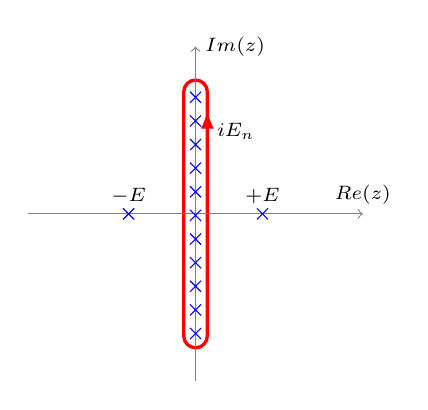
\begin{tikzpicture}
\draw[very thick, red, decoration={markings, mark=at position 0.4 with {\arrow{latex}}}, postaction={decorate}] 
      (+\w/2, -\r+\w/2) -- 
      (+\w/2, +\r-\w/2) arc [start angle=0, end angle=180, radius=\w/2] --
      (-\w/2, -\r+\w/2) arc [start angle=180, end angle=360, radius=\w/2];
\drawaxes
\drawpoles
\end{tikzpicture}
\caption{\label{fig:matsum:contourA}Contour $C_A$}
\end{subfigure}
\begin{subfigure}{0.32\textwidth}
\centering
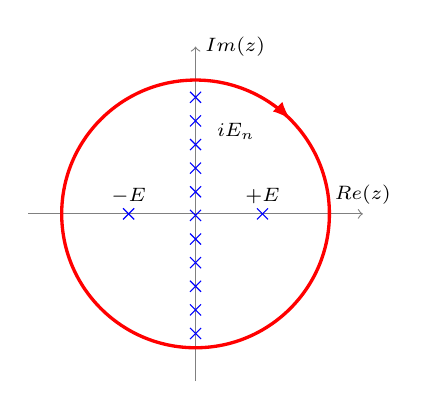
\begin{tikzpicture}
\drawaxes
\drawpoles
\draw[very thick, red, decoration={
	markings,
	mark=at position 0.125 with {\arrowreversed{latex}},
}, postaction={decorate}] (0, 0) circle [radius=\r];
\end{tikzpicture}
\caption{\label{fig:matsum:contourB}Contour $C_B$}
\end{subfigure}
\begin{subfigure}{0.32\textwidth}
\centering
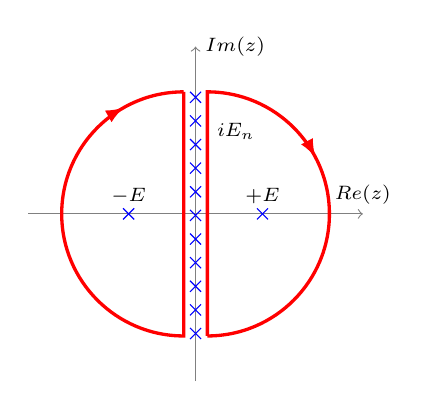
\begin{tikzpicture}
\drawaxes
\drawpoles
\draw[
	decoration={
		markings, 
		mark=at position 0.6 with {\arrow{latex}},
	}, postaction={decorate}, 
	very thick, red
] (+\w/2, -\r+\w/2) -- (+\w/2, +\r-\w/2) arc [start angle=+90, end angle=-90, radius=\r-\w/2];
\draw [
	decoration={
		markings, 
		mark=at position 0.9 with {\arrow{latex}},
	}, postaction={decorate}, 
	very thick, red
] (-\w/2, +\r-\w/2) -- (-\w/2, -\r+\w/2) arc [start angle=270, end angle=90, radius=\r-\w/2];
\end{tikzpicture}
\caption{\label{fig:matsum:contourC}Contour $C_C$}
\end{subfigure}
\caption{\label{fig:matsum:contours}%
	To evaluate a Matsubara sum \eqref{eq:matsum:sum}, we can transform it into a complex integral \eqref{eq:matsum:sum_as_contour_integral} along the contour $C_A$ that encloses infinitely many imaginary Matsubara frequencies.
	If the integral vanishes on the circular contour $C_B$ of infinite radius, we can superpose $C_B$ and $C_A$ into the contour $C_C$ that usually encloses only a \emph{finite} number of poles.
	Then we can evaluate the Matsubara sum with the residue theorem as the finite sum \eqref{eq:matsum:sum_finite_residues}.
}
\end{figure}

For reasons that will soon be clear, consider the contour integral
\begin{equation}
	\oint_{C_A} \dif z \, s(-iz) n_\pm(z)
\label{eq:matsum:contour_integral}
\end{equation}
along the contour $C_A$ drawn in \cref{fig:matsum:contourA} that surrounds all poles of $n_\pm(z)$ and is closed at $z = i \infty$ and $z = -i \infty$.
To see how it relates to the Matsubara sum \eqref{eq:matsum:sum}, first recall the \textbf{residue theorem}
\cite[theorem 1 in section 16.3]{ref:kreyszig}
\TODO{write residues as $\res_{z=z_n} f(z)$, but with $z=z_n$ \emph{below} the $\res$ symbol?, see operatorname: WikiBooks Latex Advanced Mathematics Custom Operators also do this for other operators!}
\begin{equation}
	\oint_C \dif z \, f(z) = 2 \pi i \sum_n \res[f(z_n)] ,
\label{eq:matsum:residue_theorem}
\end{equation}
where the sum runs over all poles $z_n$ of $f(z)$ inside the area enclosed by the contour $C$.
Second, recall that the \textbf{residue of a quotient function} $f(z) / g(z)$ at a simple pole $z = z_n$ where $g(z_n) = 0$, but $g'(z_n) \neq 0$ is 
\cite[equation 4 in section 16.3]{ref:kreyszig}
\begin{equation}
	\res \left[ \frac{f(z_n)}{g(z_n)} \right] = \frac{f(z_n)}{g'(z_n)} .
\label{eq:matsum:residue_quotient}
\end{equation}
Let us apply this to our integral \eqref{eq:matsum:contour_integral} with $f(z) = s(-iz)$ and $g(z) = n_\pm(z)^{-1} = e^{\beta z} \mp 1$,.
We then find that the residues of the integrand in the contour integral \eqref{eq:matsum:contour_integral} are
\begin{equation}
	\res[s(-iz_n) n_\pm(z_n)]_{z_n = i E_n} = \pm \frac{1}{\beta} s(E_n) ,
\end{equation}
By the residue theorem \eqref{eq:matsum:residue_theorem}, the contour integral \eqref{eq:matsum:contour_integral} is then
\begin{equation}
	\oint_{C_A} \dif z \, s(-iz) n_\pm(z) = 2 \pi i \sum_i \res[s(-i z_n) n_\pm(z_n)]_{z_n = i E_n}
	                                  = \pm \frac{2 \pi i}{\beta} \sum_n s(E_n)
									  = \pm \frac{2 \pi i}{\beta} S .
\label{eq:matsum:connection_integral_sum}
\end{equation}
In other words, the Matsubara sum \eqref{eq:matsum:sum} is given by the contour integral
\begin{equation}
	S = \pm \frac{\beta}{2 \pi i} \oint_{C_A} \dif z \, s(-iz) n_\pm(z) !
\label{eq:matsum:sum_as_contour_integral}
\end{equation}

What is the use of transforming a simple sum into a complex (in both senses) contour integral?
\textbf{Assume} that $s(-i z)$ -- as in our motivating example \eqref{eq:matsum:motivating_example} -- satisfies
\begin{equation}
	\abs{s(-iz) n_\pm(z)} < \frac{1}{\abs{z}} \quad \text{as} \quad \abs{z} \rightarrow \infty .
\end{equation}
Then the integral vanishes on the infinite circle contour $C_B$ in \cref{fig:matsum:contourB},
and we can superpose the contour $C_B$ on $C_A$ in the integral \eqref{eq:matsum:contour_integral} without changing its value.
Glancing back at \cref{fig:matsum:contours}, we see that this is equivalent to opening the closures in $C_A$ at $z = i \infty$ and $z = -i \infty$, and re-closing the contour with half circles in the real half planes, resulting in the contour $C_C$ in \cref{fig:matsum:contourC}.
Now we can apply the residue theorem again with the new contour $C_C$ to obtain
\begin{equation}
	S = \frac{\pm \beta}{2 \pi i} \oint_{C_C} \dif z \, s(-iz) n_\pm(z) = \mp \beta \sum_n \res[s(-iz_n) n_\pm(z_n)] ,
\label{eq:matsum:sum_finite_residues}
\end{equation}
\emph{where the sum now runs over the poles of $s(-iz)$ in the real half planes, and not the poles of $n_\pm(z)$ like in \cref{eq:matsum:connection_integral_sum}}.
Note also that the sign change following the clockwise orientation of $C_C$.
Like in our example \eqref{eq:matsum:motivating_example}, most $s(-iz)$ will have a \emph{finite} number of poles, in stark contrast to the infinite number of poles of $n_\pm(z)$.
We have thus transformed the Matsubara sum over an infinite number of residues of $n_\pm(z)$ to a sum over a finite number of residues of $s(-iz)$ -- a much more manageable task.
This is our proclaimed elegant and general method of evaluating the Matsubara sum \eqref{eq:matsum:sum}.

Let us use now use this technique to evaluate the \textbf{example} sum \eqref{eq:matsum:motivating_example} with
\begin{equation}
	s(-iz) = \frac{1}{-z^2 + E^2} .
\end{equation}
It has poles at $z = E$ and $z = -E$.
Using \cref{eq:matsum:residue_quotient} with $f(z) = n_\pm(z)$ and $g(z) = f(-iz)^{-1}$, we obtain the residues
\begin{equation}
	\res[s(-iz) n_\pm(z)]_{z =  E} = -\frac{1}{2 E} n_\pm(+E) 
	\qquad \text{and} \qquad
	\res[s(-iz) n_\pm(z)]_{z = -E} =  \frac{1}{2 E} n_\pm( E) .
\end{equation}
Using our main result \eqref{eq:matsum:sum_finite_residues}, the Matsubara sum \eqref{eq:matsum:motivating_example} is therefore
\begin{equation}
	S = \sum_{n=-\infty}^{+\infty} \frac{1}{E_n^2 + E^2}
	  = \mp \beta \sum_i \res[s(-i z_n) n_\pm(z_n)]
	  = \mp \frac{\beta}{2 E} \left( n_\pm(-E) - n_\pm(E) \right) .
\end{equation}
We can now evaluate the sum explicitly by inserting the Bose-Einstein distribution and the Fermi-Dirac distribution \eqref{eq:matsum:distribution}.
After some simplification, we obtain
\begin{equation}
	S = \sum_{n=-\infty}^{+\infty} \frac{1}{E_n^2 + E^2}
	  = \frac{\beta}{2 E} \left( 1 \pm \frac{2}{e^{\beta E} \mp 1} \right)
	  = \frac{\beta}{2 E} \left( 1 \pm 2 n_\pm(E) \right) .
\label{eq:matsum:example_result}
\end{equation}

\chapter{Integrals}

\TODO{write integrals with proofs OR references here, to keep text to the point?}

\chapter{Code}

\section{Derivation of the Tolman-Oppenheimer-Volkoff equation \texorpdfstring{\\}{} without using energy-momentum conservation}
\label{sec:tov_cas_derivation}

When deriving \cref{eq:tov} analytically, we made use of energy-momentum conservation $\nabla_\mu T\indices{^\mu^\nu} = 0$ instead of substituting our results into the unused \cref{eq:einstein_to_tov:thetatheta}.
Here, we do the latter in the computer algebra system SAGE, inspired by \cite{ref:sage_tov}.

\codefile{python}{../code/einstein_to_tov/ein.sage}

The output matches \cref{eq:tov} precisely.
